%!TEX root = mb.tex


\section{Introduction}\label{sec:intro}


    Network processing appliances (``middleboxes'') such as firewalls, NATs, proxies, and intrusion detection systems are crucial components of modern networks~\cite{aplomb,darksideofthemiddle,morley-paper}. 
     In recent trends, more and more organizations are {\it outsourcing} their network processing, either to cloud providers~\cite{aplomb, aryaka, zscalar} or to Interet service providers~\cite{attddos,comcastparentalfiltering}. 
     Network Functions Virtualization (NFV)~\cite{nfv}, which proposes moving network appliances from hardware deployments to virtualized, software deployments, makes this move increasingly attractive to service providers who can offer virtualized network features in a similar fashion to how cloud providers manage virtual servers and storage.
     For enterprise clients, this strategy promises to reduce costs, decrease the burden of managing and configuring these devices, and provide redundant resources for elasticity and fault tolerance~\cite{aplomb}.
   
   Nevertheless, outsourcing middleboxes to a third party service provider brings a new and important challenge: the confidentiality of the traffic. In order to be able to process and examine the traffic of an organization, the service provider  receives  the traffic {\em unencrypted}.  This means that the service provider now has access to potentially sensitive packet payloads,  IP addresses, and ports revealing confidential information about the organization. This situation is worrisome considering the number of documented data breaches by cloud employees or hackers gaining access to clouds~\cite{PrivacyRecords}.
   Hence, an important question is: can we enable a third party to perform traffic processing for an enterprise, {\em without seeing the enterprise's traffic}?
   
   
    We design and build \sys (read ``embark"), the first system that enables running a wide range of middleboxes at a cloud  while maintaining the confidentiality of the traffic. \sys provides these guarantees even against attackers who gained access to {\em all} the data at the cloud.  \sys's name concatenates the words MB (middlebox) and Ark (protection). 
    
    \sys encrypts traffic sent to cloud and enables the cloud to process the traffic without ever decrypting it. \sys encrypts the packet payload as well as the header (\eg{} IP addresses and ports). Since the service provider receives only encrypted traffic and no decryption key, it cannot see the confidential data. 
    Although \sys does not allow the cloud to directly read unencrypted traffic, \sys supports {\it all middlebox capabilities} typical to outsourcing environments by supporting two forms of computational encryption: {\it keyword match}, a form of searchable encryption~\cite{blindbox}, and {\it RangeMatch}.
    RangeMatch is a new encryption scheme we designed for \sys in order to enable the provider to perform prefix matching (\eg{}, if an IP address is in the subdomain 56.24.67.0/16) or port range detection (\eg., if a port is in the range 1000-2000), which are common actions performed by middleboxes such as firewalls. 
    
    Using just these two encryption schemes, we implemented a wide range of encrypted security appliances -- such as a firewall and an intrusion detection system -- as well as performance-enhancing appliances, including a WAN optimizer, a web proxy, and a load balancer. 
    Moreover, \sys supports these devices while imposing {\it zero overhead on middlebox throughput}.
    On the dataplane, middleboxes remain entirely unchanged from how they operate today: they treat encrypted packets and rules just as they treat plaintext packets and rules.
    We present a full list of the appliances \sys supports, and how it supports them, in \S\ref{sec:appliances}.


    In implementing \sys, we faced both cryptographic and systems design challenges. 

    On the algorithmic side, as we mentioned, implementing \sys required designing a new encryption scheme for {\it RangeMatch} detection.
    We required a new encryption scheme because no existing system provided both the {\it performance} and the {\it privacy} properties we desired for \sys.
    Of existing cryptographic schemes, OPE~\cite{cryptdb} is the closest relative of {\it RangeMatch}; however, it is four orders of magnitude slower than {\it RangeMatch} and leaks unnecessary information to the cloud provider.
    Where {\em RangeMatch} only reveals whether or not a value lies within a pre-determined range, OPE reveals the total ordering among all encrypted values, whether they lie within a range or not.
    We discuss the {\em RangeMatch} scheme in \S\ref{sec:rangematch} leaks unnecessary information to the cloud provider.
    %%I cut all of this discussion of homomorphic encryption -- I think Raluca has successfully sold the research community that limited, per-capabaility encryption is a good idea relative to FE or FHE. It sounds like old hat now.

\newcounter{theapp} \setcounter{theapp}{0}  
\newcommand{\capp}{\refstepcounter{theapp}\arabic{theapp}}

% 2nd fig/1st fig = 1.12 ratio
\begin{figure*}[t!]
\centering
\subfigure[Enterprise to external site communication]{
  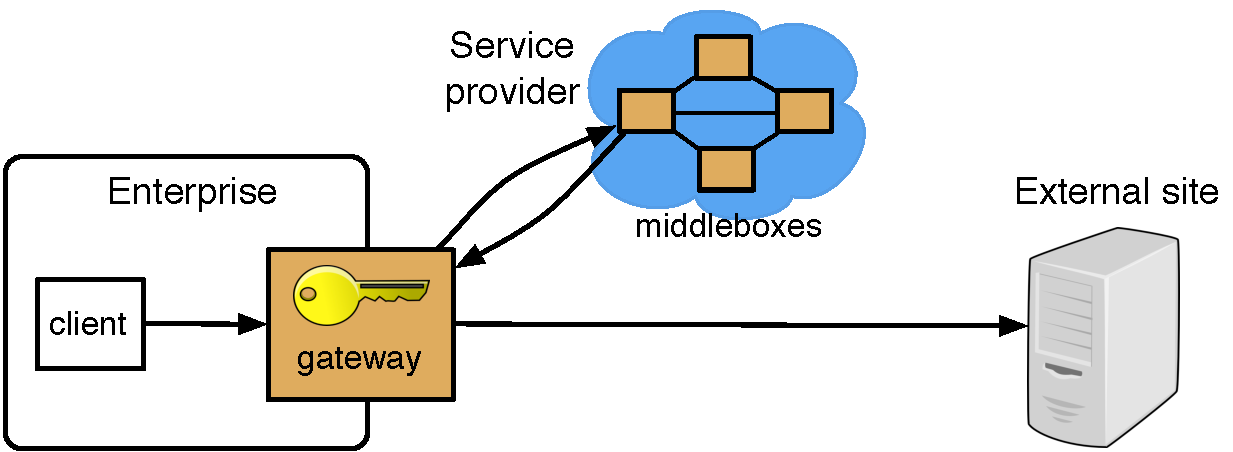
\includegraphics[width=2.8in]{fig/model_1.pdf}
  \label{fig:model1} }
%
\hfill  
\subfigure[Enterprise to enterprise communication]{
   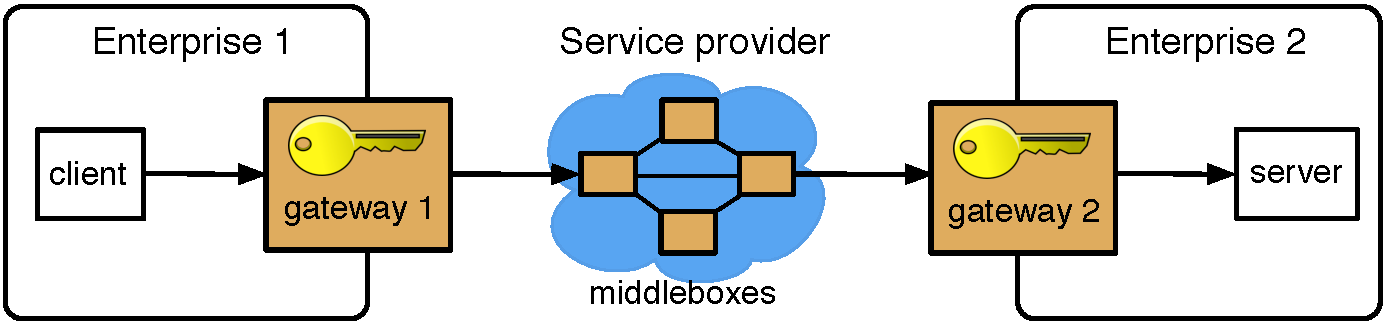
\includegraphics[width=3.2in]{fig/model_2.pdf}
     \label{fig:model2}}
     
     %
\caption{System architecture. Aplomb and NFV system setup with \sys encryption  at the gateway. The arrows indicate traffic from the client to the server; the response traffic follows the reverse direction. \label{fig:sys-overview}}
\end{figure*}


  On the systems side, \sys must be deliberate in how and where it introduces overheads due to encryption:
  
  \noindent{\it At the service provider:}
    \begin{itemize}
      \item Keep packet formats unchanged; keep dataplane unchanged. Remain compatible with state of the art classification algorithms!
      \item Almost all middleboxes require no dataplane changes, except Proxy and IDS. Although these two required changes, we need to make them as efficient as possible. Our proxy is comparable to state of the art proxy performance.
      While our IDS is based on the keywordmatch from blindbox, blindbox is too slow in setup time, and has lower security guarantees than we would like. We discuss how we improve on BlindBox in \S\ref{sec:ids}. 
      \item Minimal changes to control plane: less frequently invoked. Do require some changes to handle {\it rule updates}.
    \end{itemize}

  \noindent{\it At the enterprise:}
    \begin{itemize}
      \item Gateway: stateless
      \item Gateway: low-complexity
      \item To do otherwise would defeat the purpose of outsourcing!
    \end{itemize}


We implemented and evaluated \sys. As mentioned, we support all applications fit in the outsourcing model, as surveyed in~\cite{aplomb} -- any appliance which it outsourced today can also be outsourced using \sys.
Further, \sys imposes very negligible throughput overheads at the service provider: for example, a firewall operating over encrypted data achieves 9.8Gbps, equal to the same firewall over unencrypted data.
Our enterprise gateway can forward at 1.5 Gbps on a single core; our 8 core server can transmit \sys encrypted data at up to the full 10Gbps line rate of its network interface.
